\subsection{\label{subsecBW}Comparison to Blast-Wave model predictions}

The evolution of the \pt\ distribution with multiplicity in \pp\ collisions is remarkably similar to the evolution
observed in larger colliding systems, as underlined in Section~\ref{secResults}.
In larger systems, this evolution can be interpreted as originating from the hydrodynamical radial expansion of the produced 
medium~\cite{Abelev:2013haa,Abelev:2013vea} that can be studied by means of the Boltzmann-Gibbs Blast-Wave model (BG-BW)~\cite{Schnedermann:1993}. 
This model assumes a locally thermalized medium which expands with a
common velocity field and then undergoes an instantaneous freeze-out phase. The average expansion velocity \betaT\ and the kinematic 
freeze-out temperature \Tkin\ can be extracted with a simultaneous fit to the \pt\ distribution of several particles for each multiplicity bin and
% fitting simultaneously the \pt\ distribution of several particles at the same multiplicity and 
the result can be used to predict the \pt\ spectra of particles with different masses.\\
The result of the simultaneous BG-BW fit to $\pi$, $K$ and \p\ for the combined I+II V0M multiplicity class in \pp\ collisions at \seven\ is shown as solid lines in Fig.~\ref{fig:SpectraVsBW} (top) for the \pt\ ranges 0.5-1 GeV/$c$, 0.2-1.5 GeV/$c$ and 
0.3-3 GeV/$c$ respectively.
The predicted spectra for \kzero, \lmb, \sXi, \sOmega, \kstar\ and $\phi$ are shown as
dashed lines. The ratios between the data points and the fits or predictions are plotted in the bottom panels. Strange and multi-strange hadron spectra are reasonably 
well predicted by the BG-BW model in a \pt\ range which gets larger as the mass of the particle increases. This indicates that strange particles may
follow a common motion together with lighter hadrons and suggests the presence of radial flow even in \pp\ collisions. Resonances seem not to follow a similar expansion 
pattern, as there is no \pt\ region where the ratio data/prediction is flat. This discrepancy between BG-BW predictions and resonance 
spectra extends to all multiplicity intervals studied. 

\begin{figure*}[t!]
  \begin{flushleft}
    \center{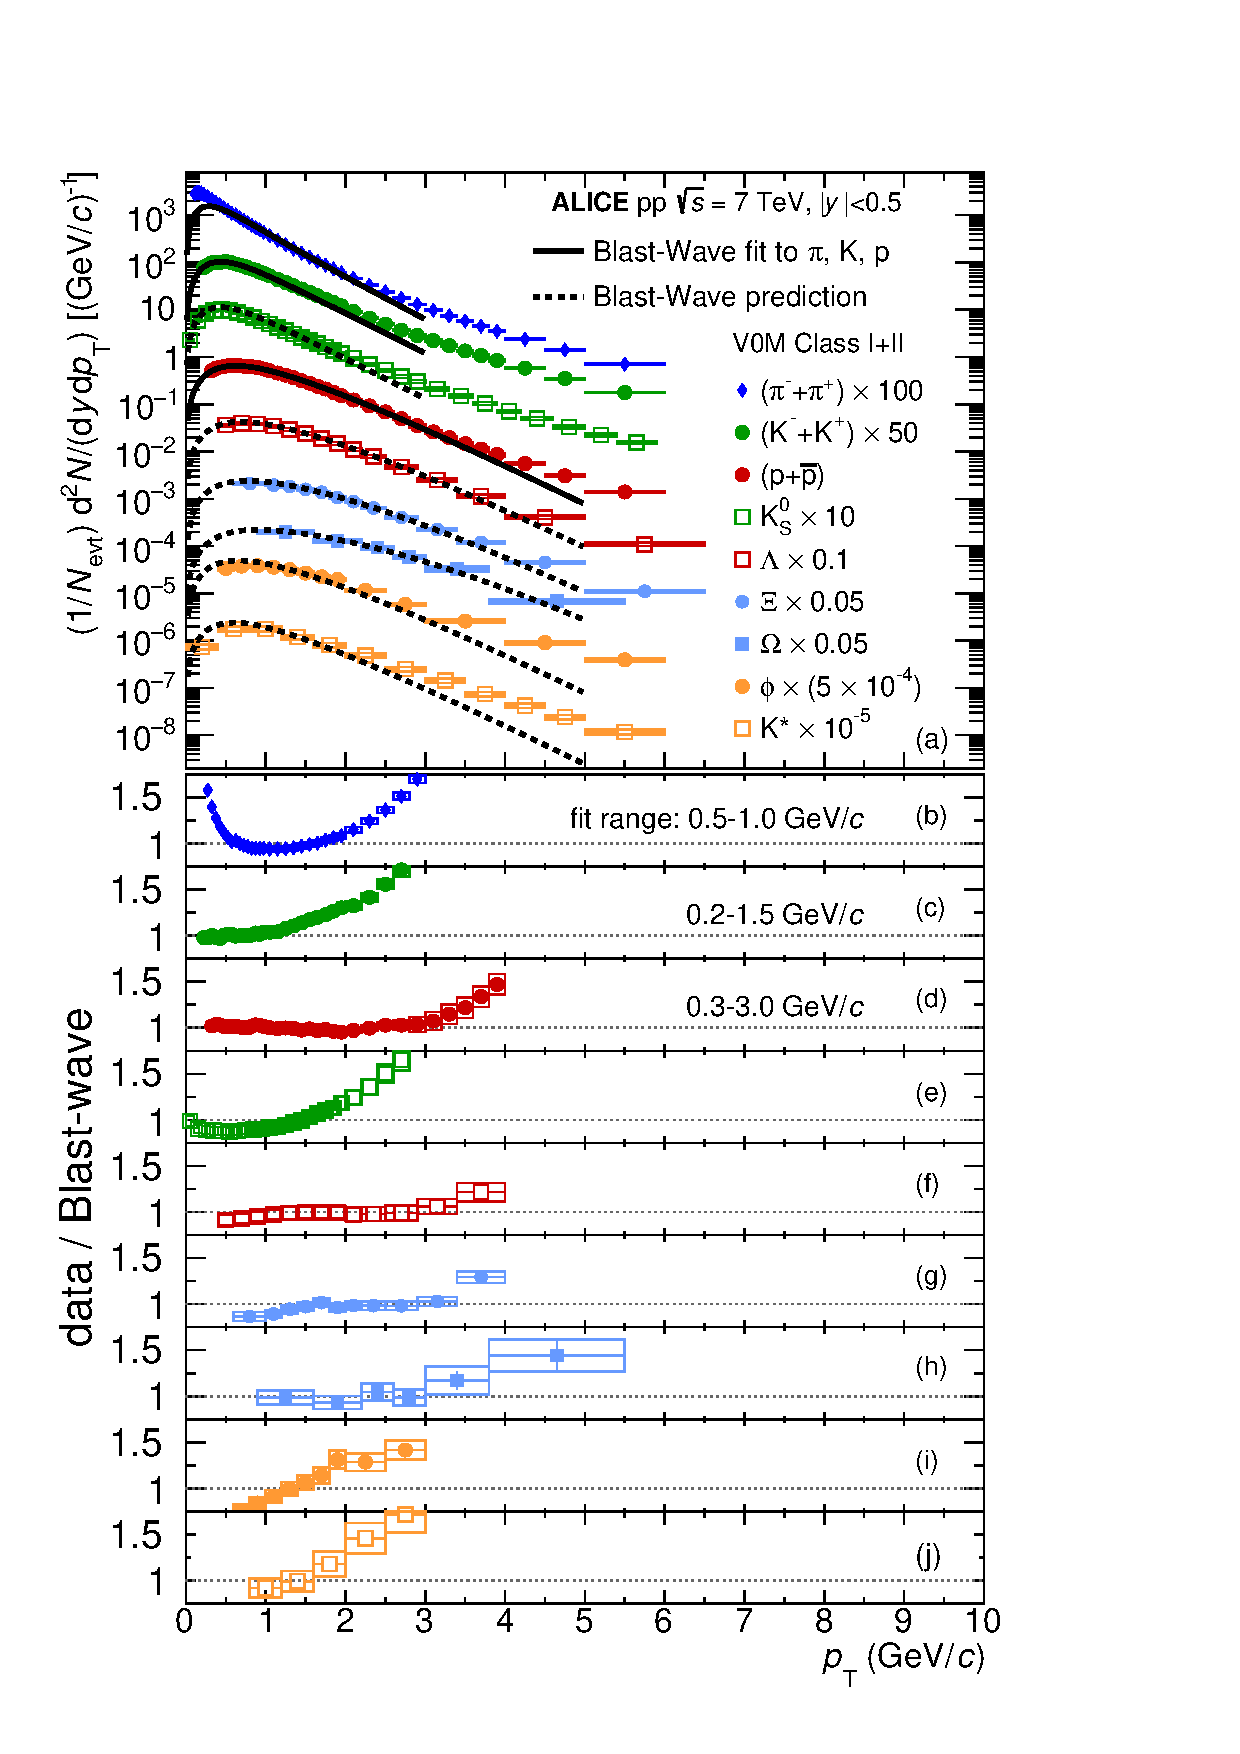
\includegraphics[width=0.605\textwidth]{figures/BlastWaveFit/img_BWfit_SpectraPrediction.pdf}}
    \end{flushleft}
    \caption{(a) Simultaneous BG-BW fit to $\pi$, $K$ and \p\ spectra from high-multiplicity (I+II V0M classes) \pp\ collisions.
             Solid lines correspond to the fit, dashed lines to the prediction. (b, c, d, e, f, g, h, i, j) Ratio data/fit(prediction) for the various
             particle species.}
    \label{fig:SpectraVsBW}
\end{figure*}  

The fit to \pp\ spectra of $\pi$, $K$ and \p\ has been performed for all the analyzed multiplicity bins and the values of \betaT\
and \Tkin\ are compared to those obtained for \pPb\ and \PbPb\ collisions in Fig.~\ref{fig:BWbetaT}. 
The fitting ranges are the same for all the three systems and a common color palette is used to highlight the average multiplicity 
corresponding to each point. Ellipses correspond to the 1-sigma contour, estimated by fitting the \pt-differential spectra with total uncertainties, i.e. after 
adding statistical and systematic uncertainties in quadrature.

Spectra in \pp\ and \pPb\ lead to very similar \betaT\ and \Tkin\ values when considering similar multiplicities, while in \PbPb\, at similar 
multiplicities, lower \betaT\ are 
observed with respect to the other two systems. This behavior has been interpreted to be a consequence of stronger radial flow gradients in the smaller 
collision systems \cite{PhysRevC.88.044915}. 

The CMS Collaboration has recently reported a similar study in~\cite{CMS:2016str}, where a BG-BW fit to the spectra of \kzero\ and \lmb\ 
has been performed for the three colliding systems, selecting the multiplicity with a central rapidity estimator. 
The \betaT-\Tkin\ progression is found to be different for \pp\ and \pPb\ collisions at high multiplicity, but the numerous differences 
with respect to the analysis discussed here (multiplicity estimator, particles included and treatment of systematic errors in the fits) 
do not allow for a quantitative comparison.

\begin{figure*}[t!]
  \begin{flushleft}
    \center{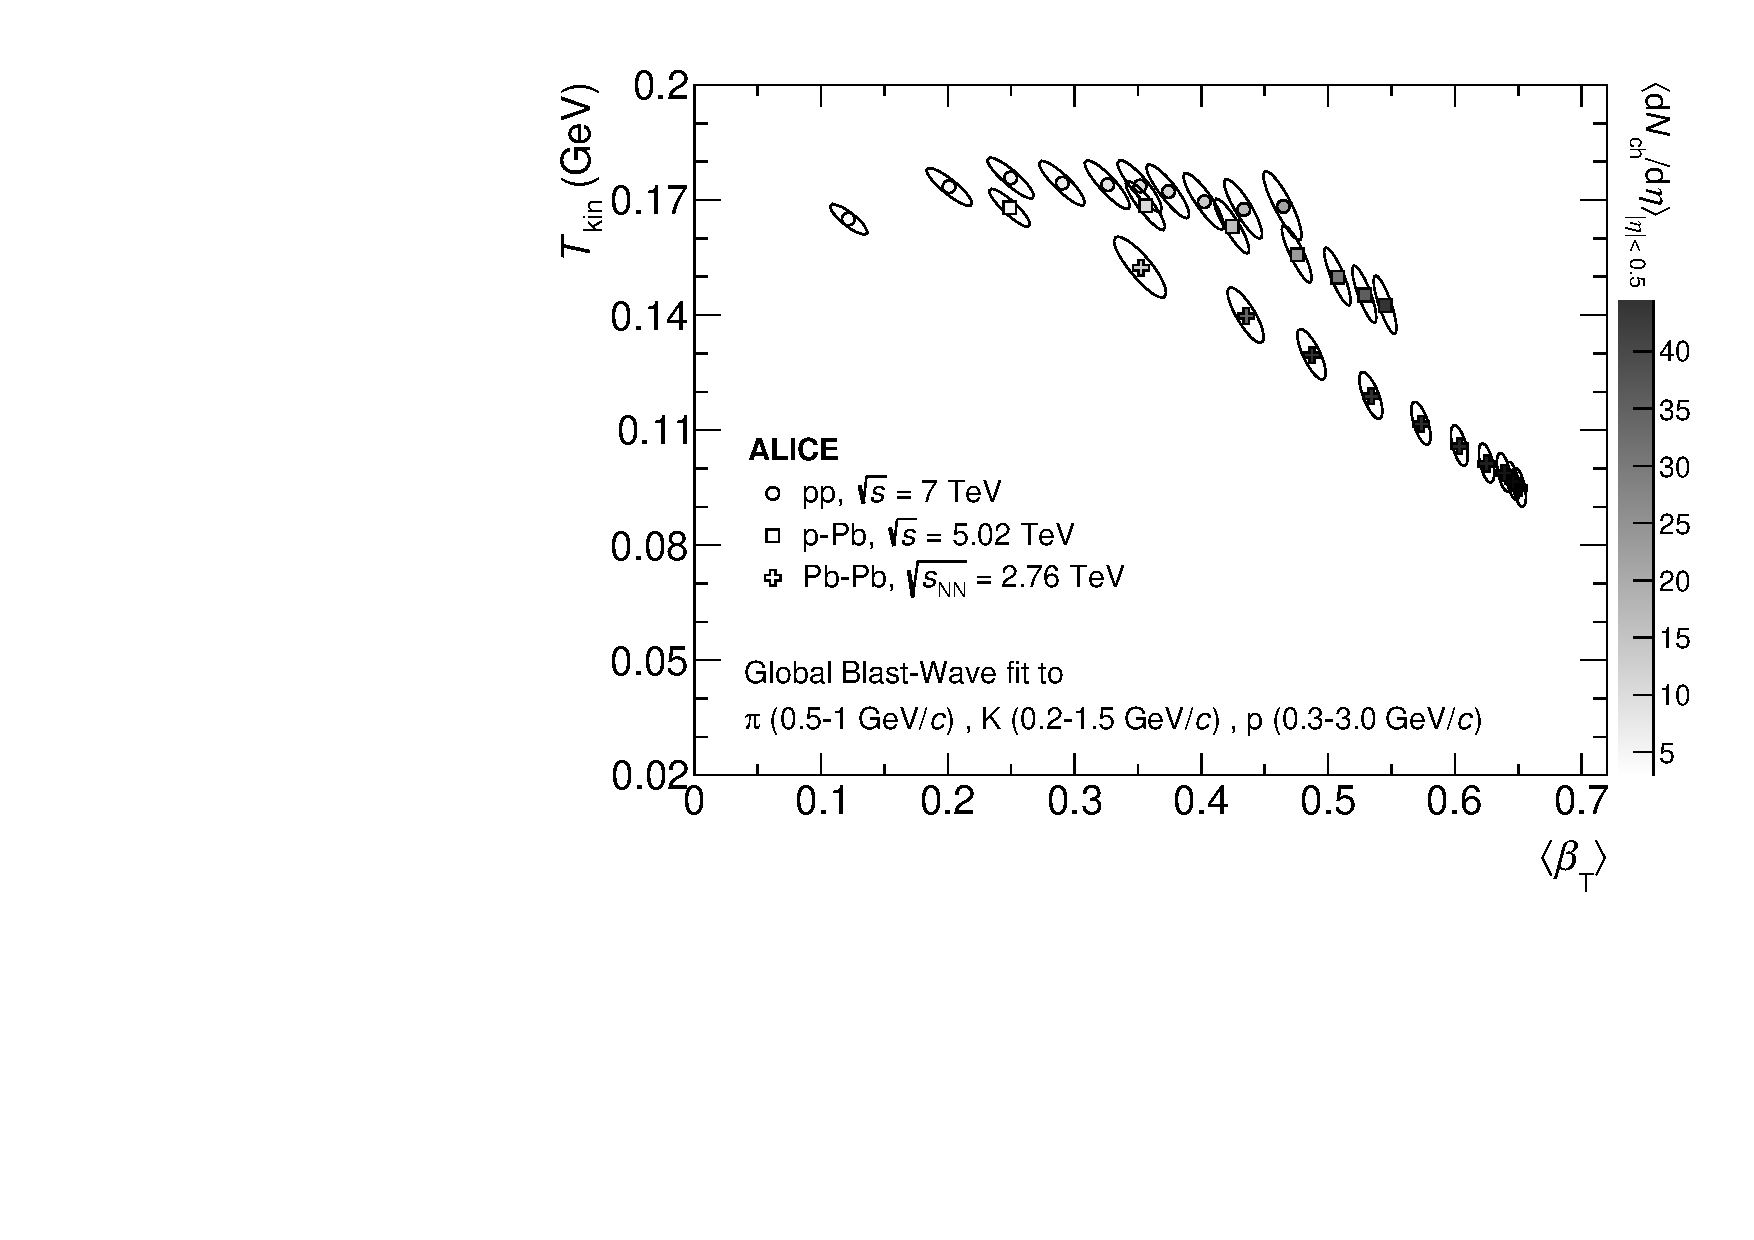
\includegraphics[width=0.69\textwidth]{figures/BlastWaveFit/img_BWfit_BetaTplot_multicol.pdf}}
    \end{flushleft}
    \caption{Kinematic freeze-out temperature parameter \Tkin\ versus average expansion velocity \betaT\ from a simultaneous BG-BW fit to $\pi$, $K$ and \p\
             spectra measured in \pp, \pPb\ and \PbPb\ collisions. The shade of the datapoints indicates the corresponding average charged-particle 
             multiplicity density.}
    \label{fig:BWbetaT}
\end{figure*}  


% \begin{figure*}[t!]
%   \begin{flushleft}
%     \center{\includegraphics[width=0.465\textwidth]{figures/BlastWaveFit/img_BWfit_TVSmult.eps}\includegraphics[width=0.465\textwidth]{figures/BlastWaveFit/img_BWfit_BetaVSmult.eps}}
%     \end{flushleft}
%     \caption{Fit of High-multiplicity pp with BW }; 
%     \label{fig:BWFitEvo}
% \end{figure*}  